37. \begin{figure}[ht!]
\center{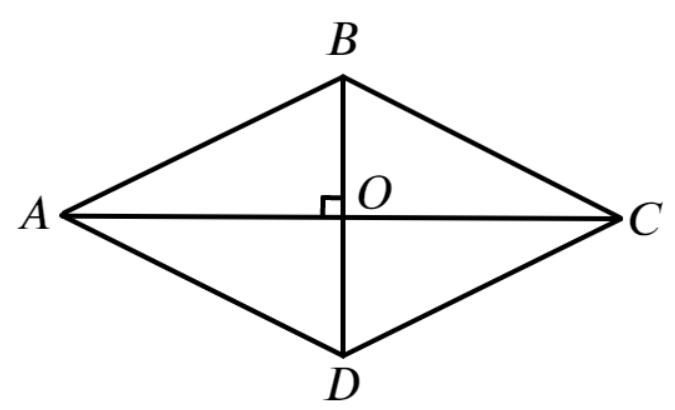
\includegraphics[scale=0.35]{g9-37.png}}
\end{figure}\\
В ромбе диагонали перпендикулярны и делятся точкой пересечения пополам. Поэтому \\$AB=\sqrt{49+576}=25$см. Найдём площадь ромба двумя способами, пусть его высота равна $h.$ С одной стороны, $S=\cfrac{1}{2}AC\cdot BD=\cfrac{1}{2}\cdot14\cdot48=336\text{ см}^2.$ С другой стороны, $S=h\cdot AB=25h.$ Значит,
$h=\cfrac{336}{25}\text{ см}.$\\
